% Options for packages loaded elsewhere
\PassOptionsToPackage{unicode}{hyperref}
\PassOptionsToPackage{hyphens}{url}
%
\documentclass[
]{article}
\usepackage{amsmath,amssymb}
\usepackage{lmodern}
\usepackage{iftex}
\ifPDFTeX
  \usepackage[T1]{fontenc}
  \usepackage[utf8]{inputenc}
  \usepackage{textcomp} % provide euro and other symbols
\else % if luatex or xetex
  \usepackage{unicode-math}
  \defaultfontfeatures{Scale=MatchLowercase}
  \defaultfontfeatures[\rmfamily]{Ligatures=TeX,Scale=1}
\fi
% Use upquote if available, for straight quotes in verbatim environments
\IfFileExists{upquote.sty}{\usepackage{upquote}}{}
\IfFileExists{microtype.sty}{% use microtype if available
  \usepackage[]{microtype}
  \UseMicrotypeSet[protrusion]{basicmath} % disable protrusion for tt fonts
}{}
\makeatletter
\@ifundefined{KOMAClassName}{% if non-KOMA class
  \IfFileExists{parskip.sty}{%
    \usepackage{parskip}
  }{% else
    \setlength{\parindent}{0pt}
    \setlength{\parskip}{6pt plus 2pt minus 1pt}}
}{% if KOMA class
  \KOMAoptions{parskip=half}}
\makeatother
\usepackage{xcolor}
\IfFileExists{xurl.sty}{\usepackage{xurl}}{} % add URL line breaks if available
\IfFileExists{bookmark.sty}{\usepackage{bookmark}}{\usepackage{hyperref}}
\hypersetup{
  hidelinks,
  pdfcreator={LaTeX via pandoc}}
\urlstyle{same} % disable monospaced font for URLs
\usepackage{color}
\usepackage{fancyvrb}
\newcommand{\VerbBar}{|}
\newcommand{\VERB}{\Verb[commandchars=\\\{\}]}
\DefineVerbatimEnvironment{Highlighting}{Verbatim}{commandchars=\\\{\}}
% Add ',fontsize=\small' for more characters per line
\newenvironment{Shaded}{}{}
\newcommand{\AlertTok}[1]{\textcolor[rgb]{1.00,0.00,0.00}{\textbf{#1}}}
\newcommand{\AnnotationTok}[1]{\textcolor[rgb]{0.38,0.63,0.69}{\textbf{\textit{#1}}}}
\newcommand{\AttributeTok}[1]{\textcolor[rgb]{0.49,0.56,0.16}{#1}}
\newcommand{\BaseNTok}[1]{\textcolor[rgb]{0.25,0.63,0.44}{#1}}
\newcommand{\BuiltInTok}[1]{#1}
\newcommand{\CharTok}[1]{\textcolor[rgb]{0.25,0.44,0.63}{#1}}
\newcommand{\CommentTok}[1]{\textcolor[rgb]{0.38,0.63,0.69}{\textit{#1}}}
\newcommand{\CommentVarTok}[1]{\textcolor[rgb]{0.38,0.63,0.69}{\textbf{\textit{#1}}}}
\newcommand{\ConstantTok}[1]{\textcolor[rgb]{0.53,0.00,0.00}{#1}}
\newcommand{\ControlFlowTok}[1]{\textcolor[rgb]{0.00,0.44,0.13}{\textbf{#1}}}
\newcommand{\DataTypeTok}[1]{\textcolor[rgb]{0.56,0.13,0.00}{#1}}
\newcommand{\DecValTok}[1]{\textcolor[rgb]{0.25,0.63,0.44}{#1}}
\newcommand{\DocumentationTok}[1]{\textcolor[rgb]{0.73,0.13,0.13}{\textit{#1}}}
\newcommand{\ErrorTok}[1]{\textcolor[rgb]{1.00,0.00,0.00}{\textbf{#1}}}
\newcommand{\ExtensionTok}[1]{#1}
\newcommand{\FloatTok}[1]{\textcolor[rgb]{0.25,0.63,0.44}{#1}}
\newcommand{\FunctionTok}[1]{\textcolor[rgb]{0.02,0.16,0.49}{#1}}
\newcommand{\ImportTok}[1]{#1}
\newcommand{\InformationTok}[1]{\textcolor[rgb]{0.38,0.63,0.69}{\textbf{\textit{#1}}}}
\newcommand{\KeywordTok}[1]{\textcolor[rgb]{0.00,0.44,0.13}{\textbf{#1}}}
\newcommand{\NormalTok}[1]{#1}
\newcommand{\OperatorTok}[1]{\textcolor[rgb]{0.40,0.40,0.40}{#1}}
\newcommand{\OtherTok}[1]{\textcolor[rgb]{0.00,0.44,0.13}{#1}}
\newcommand{\PreprocessorTok}[1]{\textcolor[rgb]{0.74,0.48,0.00}{#1}}
\newcommand{\RegionMarkerTok}[1]{#1}
\newcommand{\SpecialCharTok}[1]{\textcolor[rgb]{0.25,0.44,0.63}{#1}}
\newcommand{\SpecialStringTok}[1]{\textcolor[rgb]{0.73,0.40,0.53}{#1}}
\newcommand{\StringTok}[1]{\textcolor[rgb]{0.25,0.44,0.63}{#1}}
\newcommand{\VariableTok}[1]{\textcolor[rgb]{0.10,0.09,0.49}{#1}}
\newcommand{\VerbatimStringTok}[1]{\textcolor[rgb]{0.25,0.44,0.63}{#1}}
\newcommand{\WarningTok}[1]{\textcolor[rgb]{0.38,0.63,0.69}{\textbf{\textit{#1}}}}
\usepackage{graphicx}
\makeatletter
\def\maxwidth{\ifdim\Gin@nat@width>\linewidth\linewidth\else\Gin@nat@width\fi}
\def\maxheight{\ifdim\Gin@nat@height>\textheight\textheight\else\Gin@nat@height\fi}
\makeatother
% Scale images if necessary, so that they will not overflow the page
% margins by default, and it is still possible to overwrite the defaults
% using explicit options in \includegraphics[width, height, ...]{}
\setkeys{Gin}{width=\maxwidth,height=\maxheight,keepaspectratio}
% Set default figure placement to htbp
\makeatletter
\def\fps@figure{htbp}
\makeatother
\setlength{\emergencystretch}{3em} % prevent overfull lines
\providecommand{\tightlist}{%
  \setlength{\itemsep}{0pt}\setlength{\parskip}{0pt}}
\setcounter{secnumdepth}{-\maxdimen} % remove section numbering
\ifLuaTeX
  \usepackage{selnolig}  % disable illegal ligatures
\fi

\author{}
\date{}

\begin{document}

\hypertarget{documentation-de-lextension-optimisation}{%
\section{Documentation de l'extension
Optimisation}\label{documentation-de-lextension-optimisation}}

\tableofcontents

\hypertarget{introduction}{%
\subsection{Introduction}\label{introduction}}

Deca est un langage objet faiblement typé, à partir duquel le
compilateur Decac produit un code assembleur pour une machine
particulière. Nommé IMA, cette machine possède des performances en
cycles par instruction proche d'un microcontrôleur classique utilisé en
systèmes embarqués. Puisque ce genre de système est soumis à de fortes
contraintes, notamment en consommation d'énergie et en temps de réponse,
la réduction du temps d'exécution et de la quantité de mémoire flash
utilisée se sont rapidement révélées être d'une importance particulière
pour garantir la compétitivité de Deca. L'optimisation a donc été
intégrée dès le départ au cœur de la chaîne de compilation et garantie
de très bonnes performances sur une grande variété de programmes Deca.

Du point de vue de l'utilisateur, il est possible de choisir d'activer
ou de désactiver certaines optimisations en fonction des besoins. Il est
possible de le faire via des options ajoutées à la compilation:

\begin{Shaded}
\begin{Highlighting}[]
\NormalTok{decac {-}Ox \textless{}fichier\_source\textgreater{}}
\end{Highlighting}
\end{Shaded}

\begin{itemize}
\item
  L'option \textbf{-O0} ou aucune option engendre la compilation du
  fichier sans aucune optimisation particulière. Une bonne architecture
  de la génération de code permet d'avoir des performances tous de même
  très respectables.
\item
  L'option \textbf{-O1} fait uniquement le calcul d'expressions
  constantes à la volée. Le temps de compilation ajouté est négligeable,
  mais le gain de performance peut-être conséquent.
\item
  L'option \textbf{-O2} fait toutes les optimisations implémentées en
  utilisant un graphe de contrôle de flot. Une mise en forme SSA est
  appliquée, ce qui permet de ne n'avoir qu'une affectation par variable
  du graphe. Puis, les deux principales optimisations appliquées sur le
  graphe sont la propagation des constantes et la suppression de code
  mort. Cette optimisation n'est faite qu'à l'intérieur du main ou d'une
  méthode. Cette option permet d'avoir le gain en temps d'exécution le
  plus important, mais est aussi assez coûteuse en temps de compilation.
  De plus certaines variables peuvent être supprimées, donc l'écriture
  en mémoire du résultat n'est pas garanti.
\item
  L'option \textbf{-Og} fait les mêmes optimisations que -O2 et génère
  en plus un fichier .dot pour graphviz, afin que le graphe puisse être
  lu visuellement. Nous y reviendrons plus tard.
\end{itemize}

\hypertarget{concepts}{%
\subsection{Concepts}\label{concepts}}

Les optimisations apportées à Decac peuvent se découper en 3 parties. La
première est toujours utilisée, quelque soit l'option de compilation
choisie pour l'optimisation. La deuxième est disponible avec les options
\textbf{-O1} et \textbf{-O2}. Enfin, la dernière, qui est la plus
ambitieuse, ne s'active qu'avec l'option \textbf{-O2}.

\hypertarget{1-gestion-efficace-des-registres}{%
\paragraph{1. Gestion efficace des
registres}\label{1-gestion-efficace-des-registres}}

La machine IMA possède un nombre de registres physiques limité, au
maximum 16. Avec cette idée en tête, il devient nécessaire d'avoir une
gestion efficaces de ces registres. Dans cette optiques, il a été choisi
de ne copier une donnée en registre physique que s'il est vraiment
nécessaire de le faire. En effet, on distingue plusieurs arguments en
faveur d'une telle approche :

\begin{itemize}
\item
  La construction d'IMA garanti un faible coût des opérations mémoire,
  le fait d'en utiliser souvent n'est pas pas préjudiciable.
\item
  Le mode d'adressage d'IMA permet d'avoir, par exemple dans le cas
  d'une opération arithmétique, un des deux opérandes adressé
  indirectement. De plus, le coût d'une telle opération est le même
  quelque soit le mode d'adressage. Ainsi, il semble plus intéressant
  d'utiliser un mode indirecte face à une copie en registre physique
  lorsque cela s'avêre possible.
\item
  La présence d'immédiats dont la taille peut atteindre le mot permet de
  les utiliser très souvent, et de retarder ou supprimer les copies
  d'immédiats en registres physique.
\end{itemize}

Ainsi, l'allocation des registres a été conçue pour n'allouer des
registres physiques que si nécessaire. Une fois qu'une données est en
registre physique, elle ne peut en sortir que si elle a été libérée ou
s'il n'y a plus assez de registres pour stocker une donnée plus récente.
La politique de gestion des registres physiques est décrite plus en
détails dans \textbf{la documentation de conception, section génération
de code}.

En plus de cette politique de gestion des registres, une optimisation
supplémentaire a été ajoutée pour éviter la relecture d'une donnée qui
vient juste d'être écrite. Cette problématique apparaît dans le cas
suivant :

\begin{Shaded}
\begin{Highlighting}[]
\DataTypeTok{int}\NormalTok{ x }\OperatorTok{=}\NormalTok{ a}\OperatorTok{;}
\NormalTok{x }\OperatorTok{=}\NormalTok{ x }\OperatorTok{+} \DecValTok{1}\OperatorTok{;}
\end{Highlighting}
\end{Shaded}

En l'absence d'optimisation particulière, le code assembleur produit est
le suivant :

\begin{Shaded}
\begin{Highlighting}[]
\NormalTok{LOAD A(LB), R2}
\NormalTok{STORE R2, X(LB)}
\NormalTok{LOAD X(LB), R2}
\NormalTok{ADD \#1, R2}
\NormalTok{STORE R2, X(LB)}
\end{Highlighting}
\end{Shaded}

On remque ici que le deuxième LOAD n'est pas nécessaire car R2 contient
déjà la valeur contenue à l'adresse mémoire X(LB). Il a donc été décidé
de supprimer ce LOAD dans ce cas particulier, on obtient alors le code
suivant :

\begin{Shaded}
\begin{Highlighting}[]
\NormalTok{LOAD A(LB), R2}
\NormalTok{STORE R2, X(LB)}
\NormalTok{ADD \#1, R2}
\NormalTok{STORE R2, X(LB)}
\end{Highlighting}
\end{Shaded}

\hypertarget{2-ruxe8gles-de-ruxe9uxe9criture}{%
\paragraph{\texorpdfstring{2. Règles de réécriture
}{2. Règles de réécriture }}\label{2-ruxe8gles-de-ruxe9uxe9criture}}

Cette optimisation est présente dans le compilateur de base. L'objectif
des règles de réécriture est que c'est applicable directement sur
l'arbre au moment de la génération finale de l'arbre, à la volée.

Les règles de réécritures désignent les différentes optimisations faites
pour remplacer une instructions ou un groupe d'instructions très
coûteux. Elles ne concerne, dans le cas de Decac, que les instructions
\textbf{MUL , REM, QUO}, qui demandent beaucoup de cycles d'horloge pour
être exécutées. On a alors les règles suivantes :

\begin{itemize}
\item
  \textbf{MUL} est remplacé par une série de décalage à gauche si les
  opérandes sont de type entier, et qu'au moins un d'entre eux est un
  immédiat correspondant \(2^i\), avec \(i \in [1, 10]\) entier. on
  obtient alors, pour \textbf{4*x} :

\begin{Shaded}
\begin{Highlighting}[]
\NormalTok{LOAD X(LB), R2}
\NormalTok{SHL R2}
\NormalTok{SHL R2}
\end{Highlighting}
\end{Shaded}
\item
  \textbf{QUO} est remplacé par une série de décalage à droite si les
  opérandes sont de type entier, et que le diviseur est un immédiat
  correspondant \(2^i\), avec \(i \in [1, 10]\) entier. On obtient
  alors, pour \textbf{x/4} :

\begin{Shaded}
\begin{Highlighting}[]
\NormalTok{LOAD X(LB), R2}
\NormalTok{SHR R2}
\NormalTok{SHR R2}
\end{Highlighting}
\end{Shaded}
\item
  \textbf{REM} est remplacé par une série de décalage à droite puis à
  gauche et enfin une soustraction, si les opérandes sont de type
  entier, et que le diviseur est un immédiat correspondant \(2^i\), avec
  \(i \in [1, 5]\) entier. Dans ce cas, on applique \(i\) décalages à
  droite suivis de \(i\) décalages à gauche afin de retirer le reste de
  la dividende. Puis, une soustraction finale entre la dividende et ce
  qui vient d'être calculé permet de récupérer le reste. On obtient
  alors, pour \textbf{x\%4} :

\begin{Shaded}
\begin{Highlighting}[]
\NormalTok{LOAD X(LB), R2}
\NormalTok{SHR R2}
\NormalTok{SHR R2}
\NormalTok{SHL R2}
\NormalTok{SHL R2}
\NormalTok{SUB X(LB), R2}
\end{Highlighting}
\end{Shaded}
\end{itemize}

\hypertarget{3-calcul-dexpressions-constantes}{%
\paragraph{3. calcul d'expressions
constantes}\label{3-calcul-dexpressions-constantes}}

Cette optimisation est utilisables avec les options \textbf{-O1} et
\textbf{-O2}. Elle n'engendre pas de surcoût important sur le temps de
compilation, mais garantit un premier niveau d'optimisation intéressant.
Là aussi, c'est applicable directement sur l'arbre au moment de la
génération finale de l'arbre, à la volée.

Le calcul d'expression constantes se fait de façon récursive sur
l'arbre, il permet d'éviter d'avoir des instructions arithmétiques ou
booléennes lorsque les opérandes sont des immédiats, donc des
constantes. Un algorithme récursif permet de propager localement les
constantes à travers toute l'expression, jusqu'à ce quelle soit
entièrement calculée ou qu'une variable n'apparaisse. On obtient alors,
pour \textbf{x=1+2+3} :

\begin{Shaded}
\begin{Highlighting}[]
\NormalTok{STORE \#6, X(LB)}
\end{Highlighting}
\end{Shaded}

\hypertarget{4-contruxf4le-de-flot}{%
\paragraph{\texorpdfstring{4. Contrôle de flot
}{4. Contrôle de flot }}\label{4-contruxf4le-de-flot}}

Cette partie décrit les optimisations qui ont été implémentés grâce au
contrôle de flot. Il s'agit d'optimisations beaucoup plus ambitieuses
que les précédentes, puisqu'elles interviennent avant la génération
finale du code. La première étape consiste à transformer la liste
d'instructions en un graphe dit \emph{de contrôle de flot}. Puis un
premier traitement est appliqué sur le graphe pour le transforme en
forme \emph{SSA}, c'est à dire une forme où chaque variable n'est
affectée qu'une seule fois. Puis, deux principales optimisation sont
appliqués au graphe : la propagation de constantes et la suppression de
code mort. Enfin, le graphe est parcouru une dernière fois pour générer
le code avec les composants déjà présents.

\hypertarget{1-cruxe9ation-du-graphe-de-contruxf4le-de-flot}{%
\paragraph{1. Création du graphe de contrôle de
flot}\label{1-cruxe9ation-du-graphe-de-contruxf4le-de-flot}}

Un graphe de contrôle de flot est une représentation du programme
alternative à l'arbre abstrait. Il s'agit d'un graphe orienté, où les
nœuds contiennent une liste d'instructions exécutées linéairement, et
les arcs représentent le flot du programme. Les structures de contrôles
\emph{if} et \emph{while} engendrent des blocs ayant plusieurs arcs
sortants, un par branche. Afin d'illustrer toute l'optimisation du
contrôle de flot, un exemple de programme va être suivi durant et traité
dans les différentes sous-parties.

L'implémentation actuelle du contrôle de flot ne s'applique que sur les
blocs de code, c'est à dire l'ensemble es instructions qui composent le
main ou une méthode. Aucune gestion de contrôle de flot n'est appliquée
sur les objets ou les appels de méthodes. Cela représente néanmoins une
piste sérieuse d'amélioration possible.

Le programme traité pour l'exemple est le suivant :

\begin{Shaded}
\begin{Highlighting}[]
\OperatorTok{\{}
    \DataTypeTok{int}\NormalTok{ x }\OperatorTok{=} \DecValTok{1}\OperatorTok{;}
    \DataTypeTok{int}\NormalTok{ y }\OperatorTok{=} \DecValTok{2}\OperatorTok{;}

\NormalTok{    x }\OperatorTok{=}\NormalTok{ x }\OperatorTok{+}\NormalTok{ y }\OperatorTok{+} \DecValTok{3}\OperatorTok{;}
\NormalTok{    x }\OperatorTok{=} \DecValTok{7} \OperatorTok{*}\NormalTok{ x}\OperatorTok{;}

    \ControlFlowTok{if} \OperatorTok{(}\NormalTok{x }\OperatorTok{==} \DecValTok{42}\OperatorTok{)} \OperatorTok{\{}
        \FunctionTok{println}\OperatorTok{(}\StringTok{"la réponse est : "}\OperatorTok{,}\NormalTok{ x}\OperatorTok{);}
    \OperatorTok{\}}
    \ControlFlowTok{else} \OperatorTok{\{}
        \FunctionTok{print}\OperatorTok{(}\StringTok{"Incroyable vous êtes le 1000000e visiteur, rentrez votre numéro de carte bancaire ici pour gagner un "}\OperatorTok{);}
        \ControlFlowTok{if} \OperatorTok{(}\NormalTok{x }\OperatorTok{==} \DecValTok{38}\OperatorTok{)} \OperatorTok{\{}
            \FunctionTok{println}\OperatorTok{(}\StringTok{"weekend au ski !"}\OperatorTok{);}
        \OperatorTok{\}}
        \ControlFlowTok{else} \OperatorTok{\{}
            \FunctionTok{println}\OperatorTok{(}\StringTok{"weekend à Toulouse !"}\OperatorTok{);}
        \OperatorTok{\}}
    \OperatorTok{\}}
\OperatorTok{\}}
\end{Highlighting}
\end{Shaded}

La première étape consiste donc, à partir de l'arbre, à créer le graphe
de contrôle de flot. En le dessinant manuellement, on obtient :

\begin{figure}
\centering
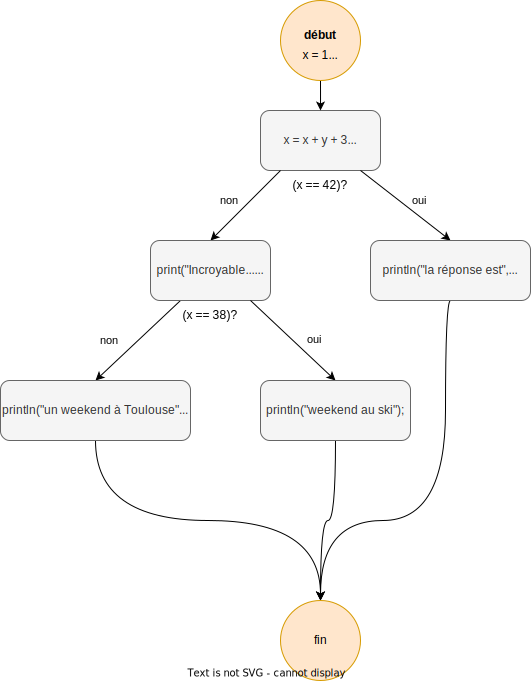
\includegraphics{/home/sylvain/Documents/ensimag/Projet_GL/gl54/docs/optimisation/graphe_debut.drawio.svg}
\caption{}
\end{figure}

Il est également possible d'obtenir ce graphe de façon automatique, en
utilisant l'option \textbf{-O2g}. Un fichier \textbf{.dot} sera alors
produit à côté des fichiers \textbf{.deca} et \textbf{.ass}. Il est
alors possible d'utiliser \textbf{graphviz} pour obtenir une image de
graphe., et l'afficher avec un visionneur d'image. Une fois le paquet
installé, la commande à utiliser est par exemple :

\begin{Shaded}
\begin{Highlighting}[]
\NormalTok{dot {-}Tsvg fichier.dot \textgreater{} fichier.svg}
\end{Highlighting}
\end{Shaded}

Pour cet exemple, le résultat est alors :

\begin{figure}
\centering
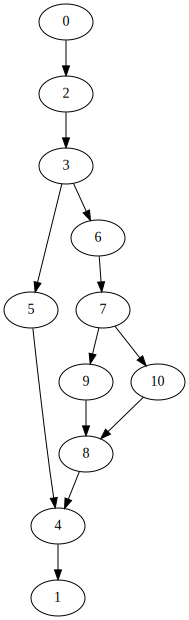
\includegraphics{/home/sylvain/Documents/ensimag/Projet_GL/gl54/docs/optimisation/doc_debut.svg}
\caption{}
\end{figure}

On retrouve alors la même structure, mais certains blocs vide ont été
ajoutés par soucis de simplification des algorithme de création du
graphe.

\hypertarget{2-mise-en-forme-ssa}{%
\paragraph{2. mise en forme SSA}\label{2-mise-en-forme-ssa}}

Il s'agit du premier algorithme appliqué au graphe nouvellement créé.
SSA signifie "Static Single Assignment" .L'objectif est de n'avoir
qu'une seul affectation de par variable. Pour cela, on notera
\textbf{\textless nom\_de\_la\_variable\textgreater\#id} chacune des
variables du programme. Le nom est celui de la variable d'origine, et
\textbf{id} est un numéro unique donnée à l'affectation unique. Pour cet
exemple, on obtient :

\begin{figure}
\centering
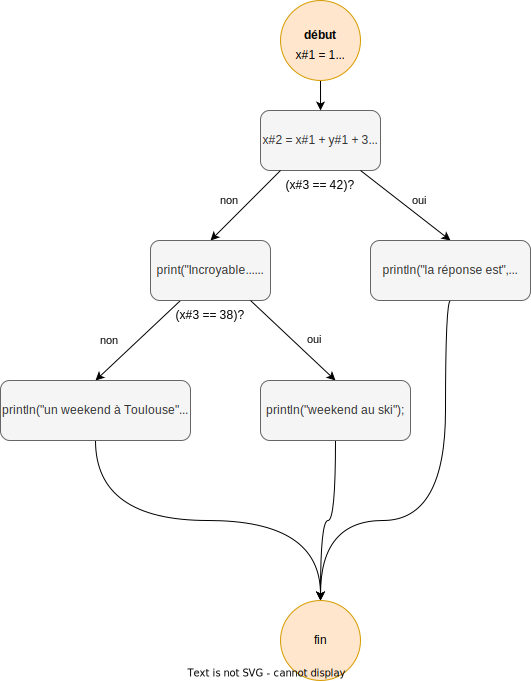
\includegraphics{/home/sylvain/Documents/ensimag/Projet_GL/gl54/docs/optimisation/graphe_ssa.svg}
\caption{}
\end{figure}

\hypertarget{3-propagation-des-constantes}{%
\paragraph{3. propagation des
constantes}\label{3-propagation-des-constantes}}

Cet étape est la première des deux optimisations principales
implémentées. Il s'agit, pour chaque variable en forme SSA, de vérifier
si l'expression qu'elle représente est une constante. Dans ce cas, on
remplace alors chacune des endroits où apparaît cette variable par la
constante associée. Puis, l'algorithme est réitéré pour toutes les
instructions qui contenaient cette variable, en recalculant les
expressions pour trouver d'autres constantes. Cela permet alors de
réduire le nombre d'instructions exécuté et donc le temps d'exécution.
Sur cet exemple, on obtient :

\begin{figure}
\centering
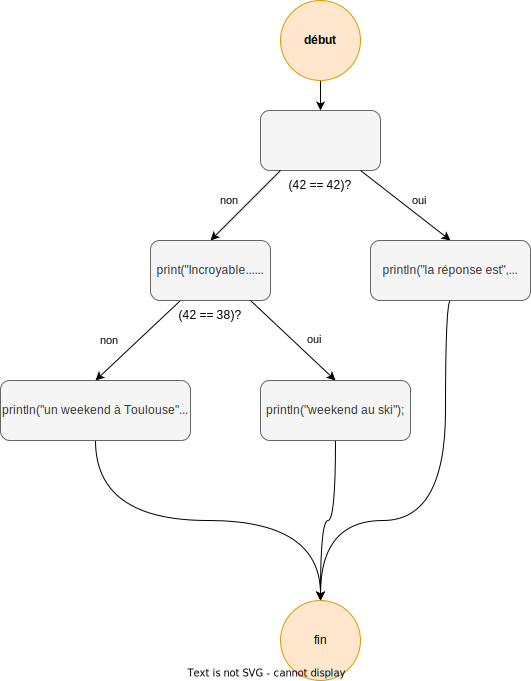
\includegraphics{/home/sylvain/Documents/ensimag/Projet_GL/gl54/docs/optimisation/graphe_constant_propagator.svg}
\caption{}
\end{figure}

\hypertarget{4-suppression-du-code-mort}{%
\paragraph{\texorpdfstring{4. suppression du code mort
}{4. suppression du code mort }}\label{4-suppression-du-code-mort}}

Cette deuxième et dernière étape de l'optimisation sur le contrôle de
flot consiste à supprimer le code rendu inaccessible. cela permet de
réduire la quantité de mémoire occupée par le résultat. Il s'agit de
tester les conditions sur les blocs possédant plusieurs arcs sortants.
Si la condition peut être évaluée sans exécuter le programme, seule la
branche prise sera conservé. On obtient alors :

\begin{figure}
\centering
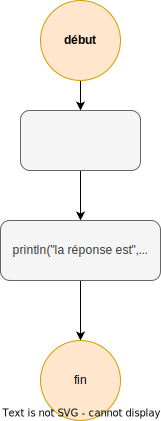
\includegraphics{/home/sylvain/Documents/ensimag/Projet_GL/gl54/docs/optimisation/graphe_fin.svg}
\caption{}
\end{figure}

En réalité il suffit de supprimer l'arc sortant vers la mauvaise branche
pour la supprimer, puisque la génération de code se fait en parcourant
le graphe. La branche non prise est alors inaccessible. Le graphe
produit par \textbf{-O2g} intègre de base cette suppression de code
mort, donc il affichera :

\begin{figure}
\centering
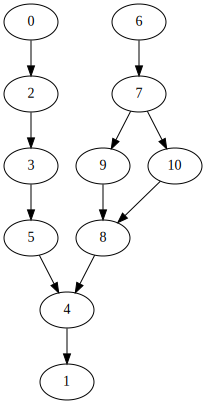
\includegraphics{/home/sylvain/Documents/ensimag/Projet_GL/gl54/docs/optimisation/doc_fin.svg}
\caption{}
\end{figure}

\hypertarget{architecture-logicielle}{%
\subsection{Architecture logicielle}\label{architecture-logicielle}}

Les deux premiers types d'optimisation présentés plus haut ont leurs
implémentations directement intégrées dans la génération de code. La
gestion des registres est notamment présentée dans la
\textbf{documentation de conception, section génération de code}. Une
exemple de règle de réécriture et le calcul d'expression constante est
aussi donnée dans la sections \textbf{Deep dive} de cette documentation.

En ce qui concerne l'optimisation par contrôle de flot, un package nommé
\textbf{opti} a été ajouté aux sources de Decac. Étant donné que
l'enchaînement des différentes étapes est linéaire, il est possible
d'obtenir une vue globale des principaux composants sous forme de
pipeline.

\begin{figure}
\centering
\includegraphics{/home/sylvain/Documents/ensimag/Projet_GL/gl54/docs/extension.drawio.png}
\caption{}
\end{figure}

\hypertarget{1-graphe-de-contruxf4le-de-flot}{%
\paragraph{1. Graphe de contrôle de
flot}\label{1-graphe-de-contruxf4le-de-flot}}

Un graphe de contrôle de flot étant un graphe orienté, il y a par
conséquence une classe \textbf{Arc}, une classe \textbf{Graphe} au sein
du package. Les blocs peuvent alors 4 types (bloc de début, bloc de fin,
bloc linéaire, bloc de branchement) qui héritent tous de la même classe
\textbf{AbstractCodeBloc}. Le graphe de contrôle de flot hérite de la
classe \textbf{Graphe} et ajoute de nombreux éléments spécifiques au
contrôle de flot.

\begin{figure}
\centering
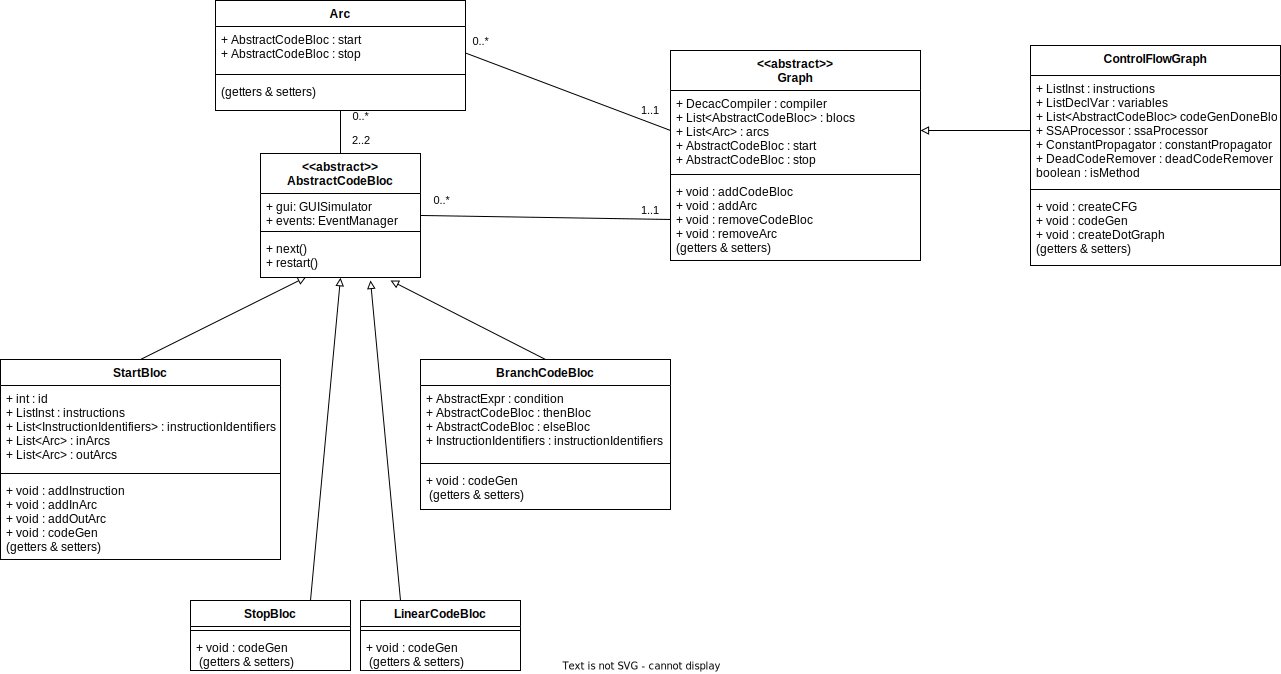
\includegraphics{/home/sylvain/Documents/ensimag/Projet_GL/gl54/docs/optimisation/graphe.svg}
\caption{}
\end{figure}

\hypertarget{2-traitement-du-graphe}{%
\paragraph{2. Traitement du graphe}\label{2-traitement-du-graphe}}

Les différents traitements à faire sur le graphe (mise en forme SSA,
propagation des constantes, suppression du code mort) sont effectuées
par des instances des classes correspondantes aux différents traitement.
Il y a donc une classe par traitement, qui sont créer et le traitement
fait dans le constructeur de \textbf{ControlFlowGraph}. Elles portent
ainsi les noms :

\begin{itemize}
\item
  SSAProcessor
\item
  ConstantPropagator
\item
  DeadCodeRemover
\end{itemize}

Les classes \textbf{Constant, SSAVariable, SSAMerge,
InstructionIdentifiers} ont été créés pour décorer le graphe ou
faciliter les différents traitements.

\begin{figure}
\centering
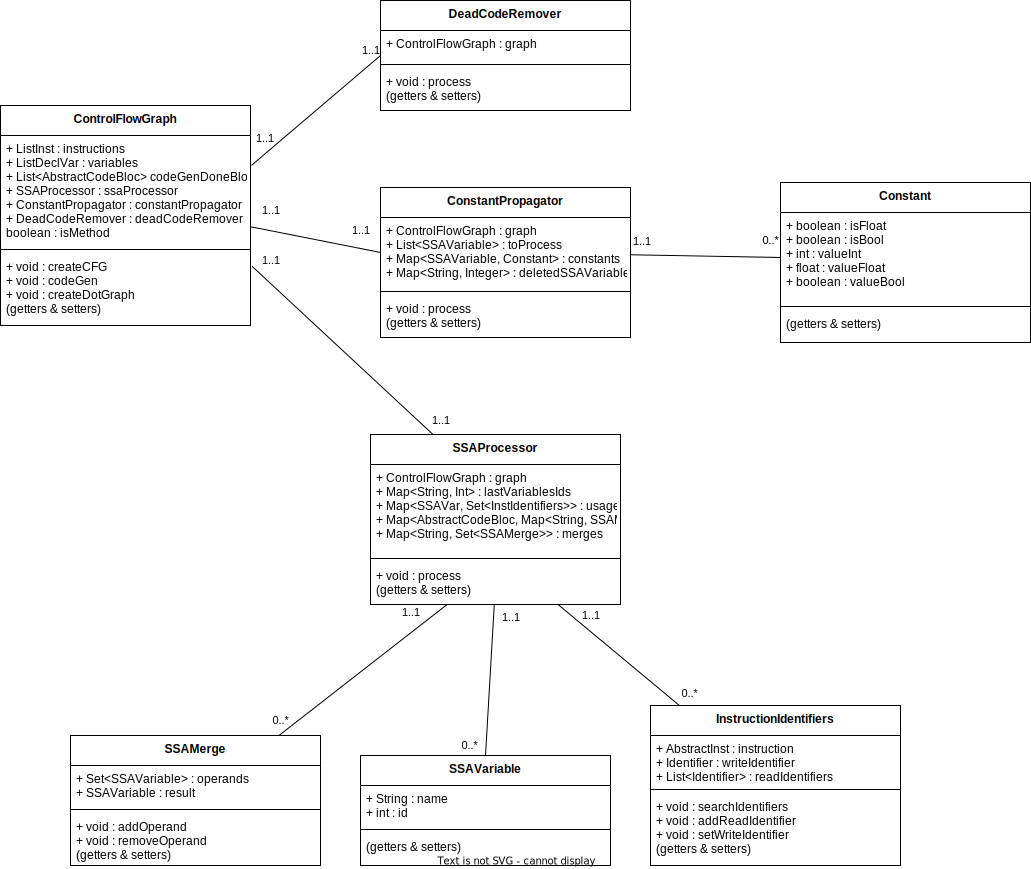
\includegraphics{/home/sylvain/Documents/ensimag/Projet_GL/gl54/docs/optimisation/processors.svg}
\caption{}
\end{figure}

\hypertarget{deep-dive}{%
\subsection{\texorpdfstring{Deep dive }{Deep dive }}\label{deep-dive}}

Alors que la section précédente se concentrais sur l'architecture des
différentes optimisations mise en œuvre, il semble intéressant d'en
expliciter certains points clés, sur lesquels repose l'implémentation
réalisée.

\begin{itemize}
\item
  \textbf{Suppression des LOAD inutiles}

  Afin d'implémenter cette optimisation détaillée dans la section
  \textbf{Concepts}, et connaissant le fonctionnement de la gestion des
  registres détaillé dans la \textbf{documentation de conception}, il a
  été nécessaire d'ajouter deux champs dans la classe
  \textbf{ContextManager} :

\begin{Shaded}
\begin{Highlighting}[]
\KeywordTok{private}\NormalTok{ VirtualRegister lastStoreRegister }\OperatorTok{=} \KeywordTok{null}\OperatorTok{;}
\KeywordTok{private}\NormalTok{ RegisterOffset lastStoreOffset }\OperatorTok{=} \KeywordTok{null}\OperatorTok{;}
\end{Highlighting}
\end{Shaded}

  Les valeur des ces champs sont modifiés à travers des setters par la
  classe \textbf{AssignOperation} juste après avoir généré l'instruction
  \textbf{STORE} d'une affectation. Ainsi, lorsque la méthode
  \textbf{freePhysicalRegister} de \textbf{ContextManager} est appelée,
  ce registre sera gardé et ne sera pas détruit. Puis, dès lors qu'une
  nouveau registre est demandé, il y a deux cas possible. Soit la donnée
  correspond à la donnée qui vient d'être stockée en mémoire, et il est
  alors possible de reprendre le registre en attente sans effectuer de
  \textbf{LOAD}, soit ce n'est pas le cas et le registre en attente est
  réellement détruit avant de créer le nouveau.
\item
  \textbf{Calcul d'expression constante}

  Cette optimisation est utilisée à deux moments. Le premier est lors de
  la propagation de constantes, le second est lors de la génération
  finale du code. Dans les deux cas, la méthode \emph{\textbf{Constant
  getConstant(DecacCompiler compiler)}} est utilisé pour cela. Présente
  dans toutes les classes héritant de \textbf{AbstractOperation} et
  \textbf{AbstractExpr} sur l'arbre, elle permet, comme la génération de
  code, de procéder récursivement sur les nœuds et jusqu'aux feuilles de
  l'arbre représentant l'expression à essayer de calculer. Pour les
  fonctions feuilles, la valeur d'un littéral remonte ainsi, et c'est
  aussi le cas pour les identifiant de variable ayant été marqué par la
  propagation de constante comme constant avec la méthode
  \textbf{setConstant}. Puis, dans le cas des opérations arithmétiques,
  booléennes, ou de comparaison, le calcul est directement effectuée
  dans le code Java, et le résultat remonte alors. Dans le cas où il
  n'est pas possible de calculer de constante, par exemple lorsqu'il y a
  des variables non connues ou une lecture d'entrée utilisateur, la
  valeur retournée est \textbf{null}.

  L'appel à la méthode \textbf{getConstant}, lors de la génération
  finale du code, est fait dans les méthodes \textbf{doOperation} des
  classes héritant de \textbf{AbstractOperation}. Si le resultat est
  différent de \textbf{null}, la constante est alors mise dans la pile
  d'opérations du \textbf{ContextManager}. Dans le cas contraire, le
  calcul est effectuée de façon classique.
\item
  \textbf{Création du graphe de contrôle de flot}

  La création du graphe de contrôle de flot est faite en appelant le
  constructeur de \textbf{ControlFlowGraph} dans la méthode responsable
  de la génération de code du \textbf{main} ou d'une \textbf{méthode}.
  De plus, il est nécessaire que l'option \textbf{-O2}. L'option
  \textbf{-O2g} va, en plus de créer le graphe, produire un fichier
  \textbf{.dot} en appelant méthode \textbf{createDotGraph}. La
  construction du graphe, à partir de la liste d'instruction, est faite
  à travers la méthode \textbf{createCFG} appelé par le constructeur de
  \textbf{ControlFlowGraph}. La liste d'instruction est alors découpée
  récursivement à chaque qu'un branchement est à ajouté, en utilisant la
  méthode \textbf{CFGRecursion}.
\item
  \textbf{Mise en forme SSA}

  Cette étape est réalisée entièrement par la classe
  \textbf{SSAProcessor}. L'appel au constructeur initialise les
  structures internes utilisées par l'algorithme principal. Ce dernier
  est exécuté lors de l'appel à la méthode \textbf{process}. Les
  structures à connaître sont les suivantes :

  \begin{itemize}
  \item
\begin{Shaded}
\begin{Highlighting}[]
\KeywordTok{private} \DataTypeTok{final} \BuiltInTok{Map}\OperatorTok{\textless{}}\BuiltInTok{String}\OperatorTok{,}\BuiltInTok{Integer}\OperatorTok{\textgreater{}}\NormalTok{ lastVariablesIds}\OperatorTok{;}
\end{Highlighting}
\end{Shaded}

    il s'agit d'une table permettant, pour une variable locale (les
    champs sont exclus et ne sont pas traités) identifiée par la chaîne
    de caractère représentant son nom, de retrouver la dernier \emph{ID}
    attribué à une variable en forme \emph{SSA}. Ce sont simplement des
    compteurs qui sont incrémentés lorsqu'une variable est à nouveau
    affectée et qu'un \emph{ID} est demander pour la variable \emph{SSA}
    produite.
  \item
\begin{Shaded}
\begin{Highlighting}[]
\KeywordTok{private} \DataTypeTok{final} \BuiltInTok{Map}\OperatorTok{\textless{}}\NormalTok{SSAVariable}\OperatorTok{,} \BuiltInTok{Set}\OperatorTok{\textless{}}\NormalTok{InstructionIdentifiers}\OperatorTok{\textgreater{}\textgreater{}}\NormalTok{ usages}\OperatorTok{;}
\end{Highlighting}
\end{Shaded}

    Il s'agit d'une table permettant, pour une variable en forme
    \emph{SSA}, de récupérer l'ensemble des
    \textbf{InstructionIdentifiers} contenant cette variable en
    particulier. Comme chaque \textbf{InstructionIdentifiers} est
    associé à une instruction, cela permet de savoir quelles
    instructions utilisent, aussi bien en lecture qu'en écriture, cette
    variable.
  \item
\begin{Shaded}
\begin{Highlighting}[]
\KeywordTok{private} \DataTypeTok{final} \BuiltInTok{Map}\OperatorTok{\textless{}}\NormalTok{AbstractCodeBloc}\OperatorTok{,} \BuiltInTok{Map}\OperatorTok{\textless{}}\BuiltInTok{String}\OperatorTok{,}\NormalTok{SSAMerge}\OperatorTok{\textgreater{}\textgreater{}}\NormalTok{ waitingFusionCodeBlocs}\OperatorTok{;}
\end{Highlighting}
\end{Shaded}

    Il s'agit d'une table permettant de stocker temporairement la liste
    des blocs à fusionner. Elle permet alors, pour un bloc en attente de
    fusion, de récupérer la table des fusions en cours associées à
    chaque variable du programme, identifiée par la chaîne de caractère
    représentant son nom.
  \item
\begin{Shaded}
\begin{Highlighting}[]
\KeywordTok{private} \DataTypeTok{final} \BuiltInTok{Map}\OperatorTok{\textless{}}\BuiltInTok{String}\OperatorTok{,} \BuiltInTok{Set}\OperatorTok{\textless{}}\NormalTok{SSAMerge}\OperatorTok{\textgreater{}\textgreater{}}\NormalTok{ merges}\OperatorTok{;}
\end{Highlighting}
\end{Shaded}

    Il s'agit d'une table permettant, pour chaque variable du programme
    identifiée par une chaîne de caractère représentant son nom,
    d'obtenir l'ensemble des fusions qui lui sont associées.
  \item
\begin{Shaded}
\begin{Highlighting}[]
\BuiltInTok{Map}\OperatorTok{\textless{}}\BuiltInTok{String}\OperatorTok{,}\NormalTok{SSAVariable}\OperatorTok{\textgreater{}}\NormalTok{ localSSA}
\end{Highlighting}
\end{Shaded}

    Il s'agit d'une structure local aux méthodes utilisées par
    l'algorithme principale. Étant donné que le graphe est parcouru de
    proche en proche, cette table est copiée et chaque copie est
    transmise aux nœuds enfants, qui vont la muter, et ainsi de suite.
    Elle permet, pour chaque variable du programme, de récupérer la
    variable en forme \emph{SSA} courante. Celle-ci est utilisée lorsque
    qu'une lecture est trouvée, et changer si une nouvelle affectation
    de la variable est détectée.
  \end{itemize}

  L'algorithme principal, dans la méthode \textbf{process}, initialise
  \textbf{localSSA} en appelant \textbf{processDeclVar}. Cela permet
  d'associer une première variable \textbf{SSA} à chaque variable
  déclarée. Puis tous les blocs sont traités de proche en proche grâce à
  la méthode \textbf{processBloc}. Il est important de bien copier
  entièrement \textbf{localSSA} si un nœud possède deux branches
  sortantes, pour rendre les copies indépendantes. La méthode
  \textbf{processBloc} a la charge de repérer les bloc avec plusieurs
  arcs entrants, qu'il faut donc fusionner. Lorsque c'est le cas, un
  opérateur souvent nommée \(\phi\) dans la littérature est à appliqué.
  Il symbolise la fusion des variables \textbf{SSA} lorsque ce ne sont
  pas les mêmes qui viennent des branches entrantes. Ici, \(\phi\) est
  représenté par la classe \textbf{SSAMerge}. Le rôle des méthode
  \textbf{startMerge, continueMerge, endMerge} appelées par
  \textbf{processBloc} lorsqu'une fusion est détectée permet que créer,
  enrichir, ou terminer les instances de \textbf{SSAMerge} nécessaires
  pour représenter toutes les fusions à faire. Par soucis de
  simplification des algorithme, une instance de \textbf{SSAMerge} est
  créée pour chaque variable, même s'il n'y a pas de conflit sur les
  deux branches. Cela évite de traiter des cas particuliers. Pour un
  exemple simple, on obtient :

  \begin{figure}
  \centering
  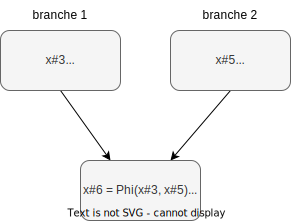
\includegraphics{/home/sylvain/Documents/ensimag/Projet_GL/gl54/docs/optimisation/SSAmerge.svg}
  \caption{}
  \end{figure}

  En réalité, ces opérateurs \(\phi\) ne possèdent pas d'implémentation
  lors de la génération finale du code. Les étapes d'optimisation
  suivantes permettent d'en supprimer une partie, lorsque les variables
  qu'ils contiennent auront été remplacées par des constantes. Ceux qui
  resteront seront traité en ne gardant qu'une case mémoire unique pour
  tous les opérandes. Ainsi, quelque soit la branche prise, la valeur
  dans cette case sera la bonne. Cela peut impacter la performances des
  processeurs de PC modernes, qui font de l'exécution spéculative, mais
  ce n'est pas le cas d'IMA.

  Enfin, pour chacune des instructions du bloc en cours de traitement,
  la méthode \textbf{processInstructionIdentifiers} est appelée avec en
  argument l'instance de classe \textbf{InstructionIdentifiers} associée
  à l'instruction, afin de traiter tous les usages de variables au sein
  de cette dernière, et ce sans avoir à reparcourir l'arbre.
\item
  \textbf{Propagation des constantes}

  L'étape de propagation des constantes est faite dans la classe
  \textbf{ConstantPropagator}. le constructeur initialise les structures
  internes et la méthode \textbf{process} permet de traiter le graphe et
  propager les constantes. Une mise en forme \textbf{SSA} du graphe doit
  être faite précédemment, car l'algorithme utilisé repose sur le fait
  que cette propriété soit vérifiée. Les structures à connaître sont les
  suivantes :

  \begin{itemize}
  \item
\begin{Shaded}
\begin{Highlighting}[]
\KeywordTok{private} \DataTypeTok{final} \BuiltInTok{List}\OperatorTok{\textless{}}\NormalTok{SSAVariable}\OperatorTok{\textgreater{}}\NormalTok{ toProcess}\OperatorTok{;}
\end{Highlighting}
\end{Shaded}

    Il s'agit d'une list, permettant de stocker temporairement toutes
    les variables en forme \emph{SSA} qu'il reste à traiter.
  \item
\begin{Shaded}
\begin{Highlighting}[]
\KeywordTok{private} \DataTypeTok{final} \BuiltInTok{Map}\OperatorTok{\textless{}}\NormalTok{SSAVariable}\OperatorTok{,}\NormalTok{ Constant}\OperatorTok{\textgreater{}}\NormalTok{ constants}\OperatorTok{;}
\end{Highlighting}
\end{Shaded}

    Il s'agit d'une table utilisée pour connaître la constante associée
    à chaque variable en forme \emph{SSA} lorsque c'est les cas. Cette
    structure est utilisée de manière conjointe avec la structure
    précédente. En effet, si une variable est détectée comme constante,
    la constante est mise dans la table et la variable dans la liste des
    variables à traiter.
  \item
\begin{Shaded}
\begin{Highlighting}[]
\KeywordTok{private} \DataTypeTok{final} \BuiltInTok{Map}\OperatorTok{\textless{}}\BuiltInTok{String}\OperatorTok{,} \BuiltInTok{Integer}\OperatorTok{\textgreater{}}\NormalTok{ deletedSSAVariables}\OperatorTok{;}
\end{Highlighting}
\end{Shaded}

    Il s'agit d'une table permettant, pour chaque variable du programme
    original identifiée par la chaîne de caractère représentant son nom,
    de retrouver le nombre de variables en forme \emph{SSA} associées
    qui ont été détruites et transformées en constantes. Si ce nombre
    est égal à \textbf{lastVariablesIds} de la classe
    \textbf{SSAProcessor}, alors toutes les variables \emph{SSA} ont été
    simplifiées, donc la déclaration et la case mémoire associées à la
    variable, peuvent êtres supprimées.
  \end{itemize}

  L'algorithme se décompose en trois parties principales. Les deux
  premières ont pour objectif de repérer les expressions constantes,
  respectivement dans les déclaration de variables et les affectations.
  Cela est fait en utilisant la méthode \textbf{getConstant} de
  \textbf{AbstractExpr} et en effectuant de nombreuses vérifications
  d'usages, relatives à la portées des variables par exemples. Les deux
  méthodes associées à cela sont \textbf{foldDeclVar} et
  \textbf{foldAssign}. Puis la troisième partie, directement codée dans
  la méthode \textbf{process} a pour rôle de propager les constantes
  précédemment calculées, de recalculer les expressions une fois la
  propagation faite, et de recommencer tant qu'il reste des variables
  \emph{SSA} à propager dans la liste \textbf{toProcess}. Une gestion
  particulière des \textbf{SSAMerge} est aussi nécessaire. La technique
  utilisée consiste à supprimer chaque opérande détecté comme constante
  des instances de \textbf{SSAMerge} associées, puis de regarder le
  nombre d'opérandes restants. S'il est égal à 0 ou 1, alors le résultat
  des totalement déterminé et la fusion peut être simplifiée. Enfin,
  lorsque la propagation est terminée, une dernière étape est faite dans
  la méthode \textbf{postProcess}, dont l'objectif est de supprimer les
  déclarations de variables devenues inutiles.
\item
  \textbf{Suppression du code mort}

  La suppression de code mort, deuxième et dernière optimisation
  implémentée, est entièrement faite dans la classe
  \textbf{DeadCodeRemover}. Plus simple que les traitements précédents,
  celui-ci ne possède qu'une méthode importante, \emph{process}, qui
  doit être appelée après avoir instancié la classe. De plus, il n'y a
  pas de structures particulière à ce traitement.

  L'algorithme consiste à parcourir le graphe de proche en proche pour
  chercher les blocs de branchement. Lorsqu'un est détectée, une
  évaluation constante de la condition est tentée, avec la méthode
  \textbf{getConstant} de \textbf{AbstractExpr}. En cas de succès, la
  branche à prendre est connue, donc il est possible transformer le bloc
  en un bloc linéaire et supprimer l'arc vers la branche inutile.
  Devenue non accessible, aucun code ne sera généré pour cette branche.
  L'algorithme s'arrête lorsque tout le graphe a été parcouru.
\item
  \textbf{Génération du code}

  Une fois les différentes optimisation de contrôle de flot faites, la
  dernière étape consiste à générer le code à partir du graphe. Pour
  cela le graphe est parcouru une dernière fois de proche en proche. A
  chaque bloc rencontré, un label sous la forme
  \emph{\textbf{Code.Bloc.xxx}} est ajouté, et les code des instructions
  est généré de façon classique. Puis, un branche conditionnel ou
  inconditionnel est ajouté vers les blocs fils en fonction de leur
  nombre. De plus, s'il n'y a qu'un bloc fils et qu'il n'a pas encore
  été traité, il n'est pas forcément nécessaire de laisse le branchement
  inconditionnel.
\end{itemize}

\hypertarget{benchmarks}{%
\subsection{Benchmarks}\label{benchmarks}}

\hypertarget{1--gain-de-performance-uxe0-lexuxe9cution}{%
\paragraph{1. Gain de performance à
l'exécution}\label{1--gain-de-performance-uxe0-lexuxe9cution}}

Afin d'évaluer le gain de performance obtenu en activant les différentes
optimisation, la première approche a été de comparer la base de tests
accumulée durant le développement de la partie en charge de la
génération de code.

Les graphiques ci-dessous montrent le gain en nombre d'instructions
totale dans le programme de sortie et en nombre de cycles IMA pour
chacun des tests utilisés :

\begin{figure}
\centering
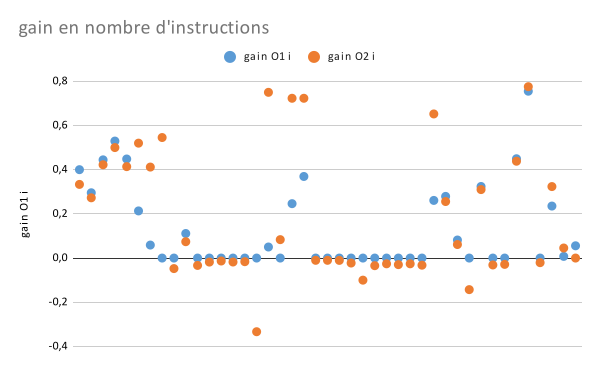
\includegraphics{/home/sylvain/Documents/ensimag/Projet_GL/gl54/docs/optimisation/gain en nombre d'instructions .svg}
\caption{}
\end{figure}

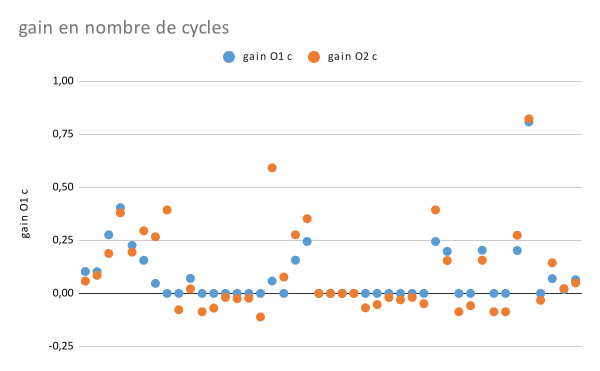
\includegraphics{/home/sylvain/Documents/ensimag/Projet_GL/gl54/docs/optimisation/gain en nombre de cycles.svg}

On observe que le gain n'est pas homogène, il dépend beaucoup du test.
En effet il faut des conditions bien particulières pour appliquer les
optimisation décrites précédemment. On remarque que l'option
\textbf{-O1} est déjà capable d'un gain très important. L'optimisation
du contrôle de flot n'a d'impact que sur un petit nombre de tests, mais
elle est aussi responsable des gains les plus importants, avec par
exemple 75\% de code en moins ou une réduction de près de moitié du
temps d'exécution sur certains tests. En revanche, plusieurs tests ont
un gain négatif en utilisant l'optimisation du contrôle de flot. En
effet certains branchements ajoutés lors de la génération de code du
graphe peuvent être responsables d'une petite baisse des performances.

En moyenne, les gains s'élèvent à \textbf{13.1\%} et \textbf{17.8\%}
pour le nombre d'instructions avec les options \textbf{-O1} et
\textbf{-O2} respectivement. Pour le nombre de cycles IMA, les gains
sont de \textbf{8.5\%} et \textbf{9.8\%} respectivement. Même si cela
semble être peu, les tests utilisés ne représentent pas bien les code
sources typiques qui peuvent être compilés avec IMA. De plus, le
compilateur de possède déjà plusieurs petites optimisations présentes de
base.

Ainsi il semble intéressant de tester les optimisation apportées sur
d'autres cas d'usages. Par chance, il existe un palmarès de performance
des compilateur de plusieurs équipes. 3 tests y sont associés. La
compilation est faite en ajoutant l'option \textbf{-n}, afin de sauter
les vérifications d'overflow par exemple (les benchmark précédents ont
été fait sans cette option). On obtient alors les résultats suivants :

\begin{figure}
\centering
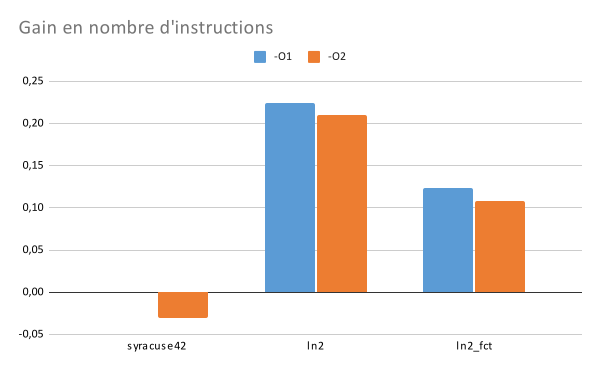
\includegraphics{/home/sylvain/Documents/ensimag/Projet_GL/gl54/docs/optimisation/Gain en nombre d'instructions perf.svg}
\caption{}
\end{figure}

\begin{figure}
\centering
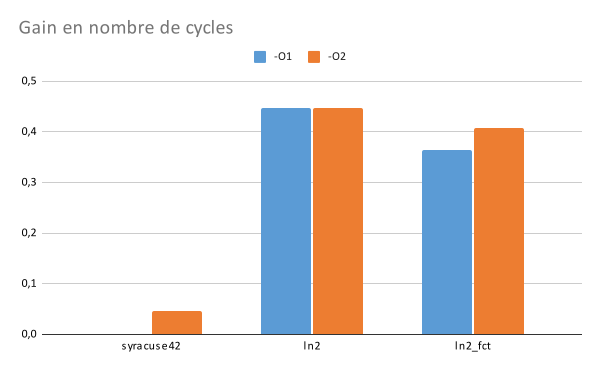
\includegraphics{/home/sylvain/Documents/ensimag/Projet_GL/gl54/docs/optimisation/Gain en nombre de cycles perf.svg}
\caption{}
\end{figure}

On observe là aussi des gains conséquent sur \emph{ln2} et
\emph{ln2\_fct}, mais le contrôle de flot n'apporte que peu de gain dans
ces cas. Pour le test \emph{syracuse42}, les grosses optimisations
étaient déjà faites par le compilateur de base, puisque la réécriture
des multiplication, division, et modulo divise par 2 le nombre de cycles
environ. Ces résultats permettent au compilateur, avec les options
\textbf{-O2 -n}, de se hisser à la 2e place du palmarès (et sans avoir
charger le résultat des tests à l'avance).

Enfin, il existe de nombreux autres cas où l'optimisation du contrôle de
flot apporte un gain très conséquent. Pour l'illustrer, l'exemple pris
dans la section \textbf{Concepts} peut être repris et tester. On obtient
alors le résultat suivant :

\begin{figure}
\centering
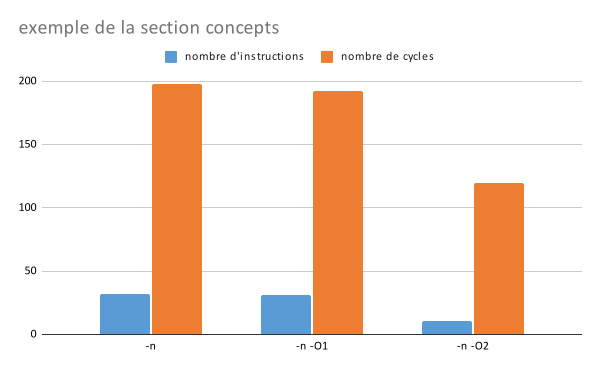
\includegraphics{/home/sylvain/Documents/ensimag/Projet_GL/gl54/docs/optimisation/exemple de la section concepts.svg}
\caption{}
\end{figure}

Dans ce cas l'option \textbf{-O1} n'a que très peu d'impact. En revanche
l'option \textbf{-O2} apporte un gain important aussi bien sur le nombre
d'instructions que sur le nombre de cycles. L'optimisation du contrôle
de flot a donc un potentiel conséquent.

\hypertarget{2-impact-sur-le-temps-de-compilation}{%
\paragraph{2. Impact sur le temps de
compilation}\label{2-impact-sur-le-temps-de-compilation}}

Pour mesurer l'impact l'impact des optimisation implémentées sur le
temps de compilation, le temps de compilation de tous le pool de tests a
été vérifié, avec les différentes options de compilations disponibles.
Les résultats n'indiquent aucune différence sortant des imprécisions de
mesures, donc il semble raisonnable de conclure que l'ajout de
l'optimisation de contrôle de flot a un impact négligeable sur le temps
de compilation.

\hypertarget{pistes-damuxe9lioration}{%
\subsection{Pistes d'amélioration}\label{pistes-damuxe9lioration}}

Même si plusieurs optimisation majeures ont été implémentées, il existe
de nombreux moyens de pousser l'optimiser plus loin. Parmi celles ci se
trouve :

\begin{itemize}
\item
  une meilleure politique de remplacement des registres. La méthode
  actuelle est proche du fonctionnement d'une pile, alors qu'une
  politique \textbf{LRU} (Last Recently Used) pourrait être une option à
  considérer.
\item
  la suppression du code pour les méthodes non utilisées
\item
  la génération du code d'une méthode courte directement dans le code
  appelant, pour évitant un appel classique coûteux.
\item
  Une meilleure évaluation des expressions constantes, en intégrant
  l'évaluation de résultats de méthodes
\end{itemize}

\hypertarget{bibliographie}{%
\subsection{Bibliographie}\label{bibliographie}}

Plusieurs sources ont été consulté pour implémentation cette extension
et réaliser cette documentation. Les principales sont les suivantes :

\begin{enumerate}
\def\labelenumi{\arabic{enumi}.}
\item
  \url{https://www.youtube.com/watch?v=uTMvKVma5ms} : il s'agit d'une
  vidéo qui a été consultée dès le départ pour apprendre dans les
  grandes lignes les concepts de l'optimisation de contrôle de flot.
  c'est la retranscription vidéo d'une conférence de \emph{Keith
  Randall}, qui a notamment implémenté plusieurs optimisations de
  contrôle de flot pour le compilateur du langage \textbf{Go}.
\item
  \url{https://en.wikipedia.org/wiki/Control-flow_graph} : la page
  wikipedia relative au graphes de contrôle de flot
\item
  \url{https://en.wikipedia.org/wiki/Static_single_assignment_form} : la
  page wikipedia relative à la mise en forme SSA
\item
  \url{https://www.cs.columbia.edu/~suman/secure_sw_devel/Basic_Program_Analysis_CF.pdf}
  : les slides d'un cours de l'université de Columbia qui permettent de
  se familiariser avec la chaîne de compilation et les graphes de
  contrôle de flot.
\item
  \url{https://pp.info.uni-karlsruhe.de/uploads/publikationen/braun13cc.pdf}
  : un papier scientifique de publié sur le site de l'université de
  Karlsruhe, qui présente une façon simple et efficace de mettre en
  forme SSA un graphe de contrôle de flot.
\end{enumerate}

\end{document}
